%-----------------------------
% CSCI 315, Spring 2018
% 
% Aaron Pfister
% Language: Ruby
%-----------------------------
% * <apfister2@mail.csuchico.edu> 2018-03-24T19:31:08.831Z:
%
% ^.

\documentclass{article}
%-----------------------------
% List of Packages 
%-----------------------------
\usepackage{graphicx}   % Need for images
\usepackage{caption}     % Useful to suppress caption numbers with *
\usepackage{listings}      % Needed for code and syntax highlighting
\usepackage{multicol}     % Permits sections with multiple columns
\usepackage{enumitem}  % More options for itemize, enumerate, and description
\usepackage{hyperref}            % For nice urls
\usepackage{tikz}            % For drawing cool things

%-----------------------------
% Set Settings and Macros
%-----------------------------

% define some custom colors
\definecolor{comment_green}{rgb}{0,0.6,0}
\definecolor{numbers_gray}{rgb}{0.5,0.5,0.5}
\definecolor{string_mauve}{rgb}{0.58,0,0.82}

% This is the default columnsep (from multicolums)
\setlength\columnsep{30pt} 

% Configure code and syntax highlighting
% Not all languages supported (but many are)
% Find the language closest to yours, and extend it with morekeywords
% Recommended reference: https://en.wikibooks.org/wiki/LaTeX/Source_Code_Listings
\lstset{%
    language=Ruby,   
    basicstyle=\small,                                          % the size of the fonts that are used for the code
    commentstyle=\color{comment_green},       % comment style
    keywordstyle=\color{blue},                          % keyword style
    morekeywords={*,...},                                 % if you want to add more keywords to the set
    stringstyle=\color{string_mauve},                % string literal style
    numberstyle=\tiny\color{numbers_gray},        % the style that is used for the line-numbers
    numbers=left,                                            % where to put the line-numbers; possible values are (none, left, right)
    numbersep=6pt,
    frame=single, % adds a frame around the code
    keepspaces=true,
    tabsize=2	                                                     % sets default tabsize to 4 spaces
}

\begin{document}
%-----------------------------
% Header
%-----------------------------
\title{Ruby Lab Proposal: D\&D Dice Roller \\ \large{\sc CSCI 315, Programming Languages}}
\author{Aaron Pfister}
\date{Spring 2018}
\maketitle
% Use tikz to add some images outside the normal printing area
\begin{tikzpicture}[remember picture,overlay]
   % This sets logo in upper right corner (optional)
   \node[anchor=north east,inner sep=40pt] at (current page.north east)
             {
\includegraphics[scale=0.36]{ddo2}};
   \draw (-4,1) -- (15,1);
\end{tikzpicture}

%-----------------------------
% Overview
%-----------------------------
\section*{Overview}
The goal of this lab is to create a 2 player (Human vs. Machine, Human vs. Human, Machine vs. Machine), turn based dice rolling game. My inspiration for this lab comes from turn based video games and a dungeons and dragons video game I used to play. I also believe the turn based style is easier to think about, plan and implement in code. Since Ruby is object-oriented, this lab will utilize classes and inheritance. 

\subsection*{Vision}
My vision for this lab starts with a Dungeons and Dragons type picture printing along with a prompt asking the user to pick Player 1 and Player 2. From this point, initialization of weapons and their damage can occur. After the players have been selected and the weapons initialized, the game is ready to be played. For now, a game will consist of 3 rounds with 1 ranged round and 2 melee rounds, and I may add the possibility of more rounds (i.e. 5 rounds with 2 ranged and 3 melee and 7 rounds with 3 ranged and 4 melee). The beginning of each round will start with a picture and prompt asking each player to choose their weapon for the round (the computer class will pick automatically). Once both players are ready, the turn based system comes in: one at a time, back and forth, the players call their swing() or shoot() functions to determine the damage they deal to their opponent. After each turn, the outcome of their swing() or shoot() should be printed along with the updated health of the opponent. At the end of each round, the winner of the round will be printed. At the end of the game (all rounds completed), a picture will be printed to the screen along with a summary of the rounds followed by the winner of the game. I will provide pictures to print at various points throughout the program, but you are able to substitute any picture for boosting the experience.  

\subsection*{Player Class}
The player class will hold the name of the player. In this lab, you will use \textbf{attr\_accessor} to automatically make getter and setter methods. This class will also hold the hit points (health bar) for each player \cite{code:blog}.
\begin{enumerate}

\item \textbf{Computer:} Controlled by the computer, randomly picks 2 weapons (melee and ranged) when initialized. After the first round, it will pick a new weapon at the beginning of each round. Define the swing() method to call the weapons and return a miss or the damage dealt. 

\item \textbf{Human:} The Human player will hold the weapons chosen by the user. Define the swing() method to call the weapons and return a miss or the damage dealt. Note: the math for the swing methods may differ.

\end{enumerate}

\subsection*{Weapon Class}
The Weapon class will contain a name along with the type (melee/ranged). Again, you will use \textbf{attr\_accessor} to automatically create getter and setter functions.

\begin{enumerate}

\item \textbf{Melee (Longsword, Mace, Rapier):} The melee class will hold to hit and damage modifiers for the weapon. Damage modifiers use the "1d10" syntax to determine the number of sides on the dice and the multiplier (unique for each weapon). I am debating how to calculate the to hit modifier to make the game a little more interesting. I am also thinking of a critical multiplier for both melee and ranged weapons, but do not know how the game flow will be before adding this. This class will implement the swing() method, which will determine if the weapon hits, and if it does, how much damage it did. 

\item \textbf{Ranged (Short bow, Light Crossbow):} The ranged class will also hold to hit and damage modifiers for the weapon. The ranged weapons critical multiplier (if there is one) will be based on how many consecutive hits that player has gotten. This class will implement the shoot() method, which determines if the shot hits, and if it does, how much damage it did.

\end{enumerate}

\subsection*{Input}
The input of this lab will consist of the damage modifiers for each of the 5 weapons. I am still thinking about making the to hit (and possibly critical multiplier) hard coded or different from test to test. Player 1 and Player 2 will be chosen via the prompt, and then the choice of weapon at the beginning of each round will be given.

\subsection*{Output}
The output should contain the "play by play" of each round along with the announcement of the winner. After 3 rounds, the summary of each round along with the final winner should be displayed. Something along the lines of:
\begin{lstlisting}
------Picture that signifies a round has started-----
Player 1 swung their longsword for 22 damage
Player 2 health went down to 73
Player 2 swung their rapier for 16 damage
Player 1 health went down to 52
Player 1 missed!
...
Player 1 ran out of health
Player 2 won the round!
\end{lstlisting}
\begin{lstlisting}
Player 1 defeated Player 2 in a ranged match
Player 2 defeated Player 1 in a melee match
Player 1 defeated Player 2 in a melee match
Player 1 wins the game!
\end{lstlisting}

%-----------------------------
% Lab Difficulty
%-----------------------------
\section*{Lab Difficulty}
\begin{description}[noitemsep]
\item [Medium:] This lab requires some understanding of object oriented programming and searching for information beyond what is given in the prompt. For most students doing this lab, I am assuming they know little to nothing about Ruby. Just as in the Python lab, some web research learning syntax and the language will be necessary to complete the lab.
\end{description}

%-----------------------------
% Showing Off The Language
%-----------------------------
\section*{Showing Off Ruby} 

\begin{enumerate}

\item \textbf{Classes} will be required to show off the Object Oriented paradigm in Ruby. For example, the use of a Weapon parent class will allow you to create different types of melee and ranged weapons. 

\item \textbf{Modules!} Modules allow you to create methods that can be used by different classes. You are not allowed to make an instance of a module; modules are static. Modules give you the ability to move logic and hard to read code to a different location, thus making your methods more readable.

\item \textbf{Ruby Gems!} This lab will use the 'catpix' gem for displaying pictures into terminal. Although the pictures cannot be very detailed, it is an extremely easy way to print a .png, .jpg, etc. and will to the "feel" of the game

\end{enumerate}
\newpage

%-----------------------------
% Testing
%-----------------------------
\section*{Testing} 
For testing, the student may use the piping methods for inputing files and printing output to files. The catpix pictures do not come out well in the .out files, but I checked to make sure the files still work with the vimdiff utility. As of now, I do not have a way of implementing the Tyson run\_tests, but you are able use and test each test on an individual basis.

%-----------------------------
% Code Examples
%-----------------------------
\section*{Code Examples } 

\subsection*{Using Modules \cite{code:beginners}}
\begin{lstlisting}
require 'digest'

module Encryption
  def encrypt(string)
    Digest::SHA2.hexdigest(string)
  end
end

class Person
  include Encryption
  # ...
  def encrypted_password
    encrypt(@password)
  end
end

person = Person.new("Ada")
person.password = "super secret"
puts person.encrypted_password
\end{lstlisting}

\subsection*{Catpix \cite{code:github}}
With only a 9 lines of code:
\begin{lstlisting}
require 'catpix'

Catpix::print_image "sunglass.png",
  :limit_x => 0.7,
  :limit_y => 0,
  :center_x => true,
  :center_y => true,
  :bg => "white",
  :bg_fill => false,
  :resolution => "high"
\end{lstlisting}
\newpage
I can print this into terminal:
\begin{center}
    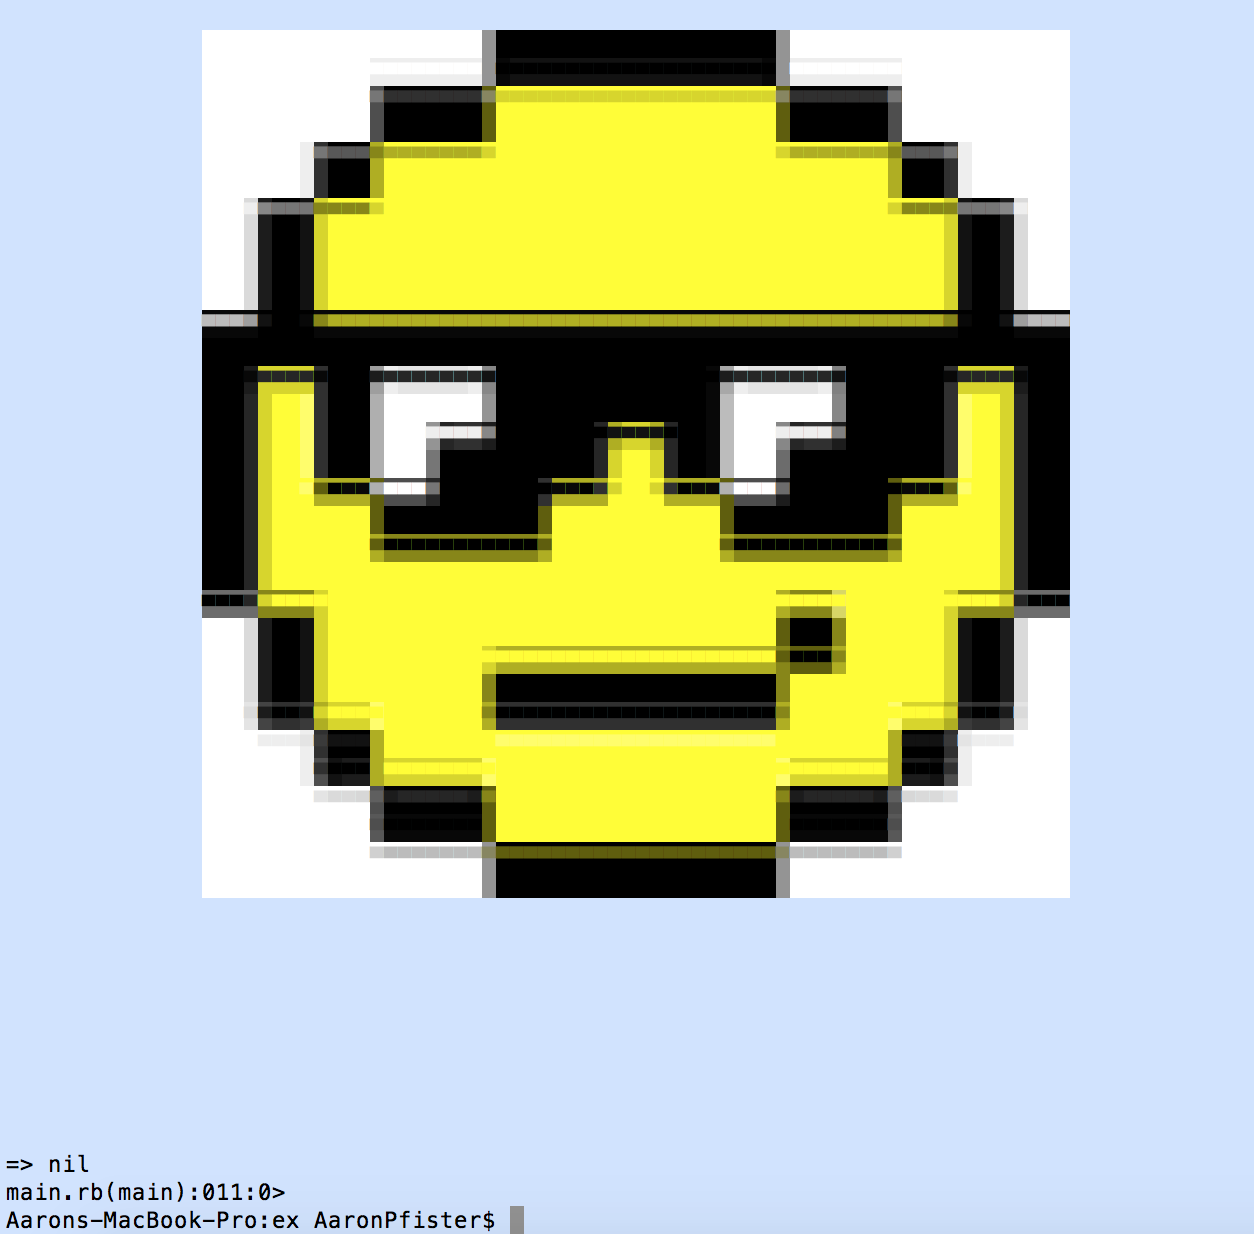
\includegraphics[width=0.7\textwidth]{output}
\end{center}
\newpage

%-----------------------------
% References (Required)
%-----------------------------
\bibliographystyle{plain}
\bibliography{ruby}      % matches perl.bibs

\end{document}
